\documentclass[
BCOR0.7cm,							% Bindekorrektur, bspw. 1 cm
]
{scrbook}

\newif\ifpdf
\ifx\pdfoutput\undefined
	\pdffalse              	%normales LaTeX wird ausgef�hrt
\else
	\pdfoutput=1           
	\pdftrue               	%pdfLaTeX wird ausgef�hrt
\fi

\ifpdf
	%\usepackage{ae}        % Benutzen Sie nur
	%\usepackage{zefonts}  	% eines dieser Pakete
\else
	%%Normales LaTeX - keine speziellen Fontpackages notwendig
\fi

\ifpdf %%Einbindung von Grafiken mittels \includegraphics{datei}
	\usepackage[pdftex]{graphicx} %%Grafiken in pdfLaTeX
\else
	\usepackage[dvips]{graphicx} %%Grafiken und normales LaTeX
\fi


\ifpdf
	\pdfinfo
	{
    /Author (Andreas �sterreicher)                                
    /Title (Inventar)     
    /Subject (Inventar)
    /Keywords (INVENTAR FH-Complete Technikum-Wien)
	}
\else			
\fi

\usepackage{listings} \lstset{numbers=left, numberstyle=\tiny, numbersep=5pt}
\lstset{language=tex} 


\usepackage[pdftex,colorlinks=true,urlcolor=blue,linkcolor=blue]{hyperref}
\usepackage[ngerman]{babel}		
\usepackage[T1]{fontenc}
\usepackage[latin9]{inputenc}
\usepackage{makeidx}
\usepackage{float}
\usepackage[small,bf]{caption}
\usepackage{fancyhdr}
\usepackage{amssymb,amsmath}
\makeindex

\graphicspath{{../../images/}}

\setlength{\tolerance}{2000}
\setlength{\parindent}{0pt}
\setlength{\parskip}{1ex plus 0.5ex minus 0.2ex}
\addtolength{\textheight}{2cm}
\addtolength{\headheight}{2pt}
\setlength{\captionmargin}{20pt}
\floatstyle{plain}
\floatname{example}{Example}

\newfloat{example}{hbtp}{loe}[chapter]
\floatplacement{figure}{hbtp}
\floatplacement{table}{htbp}

\newcommand{\dollar}{\char36}

\newenvironment{info}[1]{
    \hspace{-10mm}
    \fbox{
        \begin{minipage}{1cm}
        
\includegraphics[width=1cm]{icon_info}
        \end{minipage}
        \begin{minipage}{14.5cm}
        #1
        \end{minipage}
    }
}

\newenvironment{achtung}[1]{
    \hspace{-10mm}
    \fbox{
        \begin{minipage}{1cm}
        
\includegraphics[width=1cm]{icon_achtung}
        \end{minipage}
        \begin{minipage}{14.5cm}
        #1
        \end{minipage}
    }
}

\newenvironment{halt}[1]{
    \hspace{-10mm}
    \fbox{
        \begin{minipage}{1cm}
        
\includegraphics[width=1cm]{icon_halt}
        \end{minipage}
        \begin{minipage}{14.5cm}
        #1
        \end{minipage}
    }
}

\newenvironment{idee}[1]{
    \hspace{-10mm}
    \fbox{
        \begin{minipage}{1cm}
        
\includegraphics[width=1cm]{icon_idee}
        \end{minipage}
        \begin{minipage}{14.5cm}
        #1
        \end{minipage}
    }
}


\setlength{\unitlength}{1mm}

\newenvironment{markier}[5]{
    
    \thicklines \put(#2,#3){\vector(#4,#5){5}} \thinlines
    \put(#2,#3){\circle*{5}}
    \put(#2,#3){\textcolor{black}{\circle{5}}\makebox(-10,0){\textcolor{white}{#1}}}


}


\hyphenation{gleich-zeitig para-meter}


\begin{document}

\ifpdf
	\DeclareGraphicsExtensions{.pdf,.jpg,.png}
\else
	\DeclareGraphicsExtensions{.eps}
\fi

\pagestyle{fancyplain}
% Titelseite einbinden
%
% Titelseite, Abstrakt, Danksagung und Inhaltsverzeichnis
%
%% eigene Titelseitengestaltung %%%%%%%%%%%%%%%%%%%%%%%%%%%%%%%%%%%%%%%    

\begin{titlepage}
\begin{center}
\vspace*{40mm} \huge Inventar-Handbuch\\
\vspace*{10mm}
\large 

\vfill 
\includegraphics[width=130mm]{fhcomplete}
	
\vfill \textsc{Fachhochschule Technikum Wien}\\

Wien, \today
\end{center}
\end{titlepage}


\tableofcontents			% Inhaltsverzeichnis
\frontmatter					% Vorspann (z.B. r�mische Seitenzahlen)
\chapter{Einleitung}
Im folgenden wird die Funktionalit�t der Inventarverwaltung des FH-Complete Softwarepaketes beschrieben.\\
Dies umfasst die Verwaltung, Inventariesierung und Inventur von Betriebsmitteln jeglicher Art.\\
\\
Die Inventarverwaltung ist auf den Betrieb mittels Barcodescanner ausgelegt.
\mainmatter						% Hauptteil

%% Kapitel Anfang %%%%%%%%%%%%%%%%%%%%%%%%%%%%%%%%%%%%%%%%%%%%%%%%%

\chapter{Neues Betriebsmittel anlegen}
\label{Neues Betriebsmittel anlegen}
�ber den Men�punkt Inventar->Neu k�nnen neue Betriebsmittel angelegt werden.
Werden mehrere gleiche Betriebsmittel angelegt, kann eine Vorlage verwendet werden. In diesem Fall m�ssen nur die Daten ge�ndert werden die sich pro Ger�t unterscheiden (etwa Inventarnummer und Seriennummer).\\
Dazu kann in der Auswahlbox im Kopfbereich des Formulares die Anzahl der anzulegenden Betriebsmittel ausgew�hlt werden.
Die eingetragenen Daten werden automatisch f�r die einzelnen Betriebsmittel �bernommen.\\
\\
Die Inventarnummer wird nicht vom System generiert! Diese wird vom Programm des Etikettendruckers erstellt und h�ndisch oder mittels Barcodescanner eingetragen.
Die Details zu den einzlnen Betriebsmitteln k�nnen �ber den Punkt 'Inventardaten anzeigen/ausblenden' angezeigt werden.
Der klick auf einen der 'speichern' Buttons speichert immer alle der angezeigten Betriebsmittel.
\begin{figure}
	\centering
	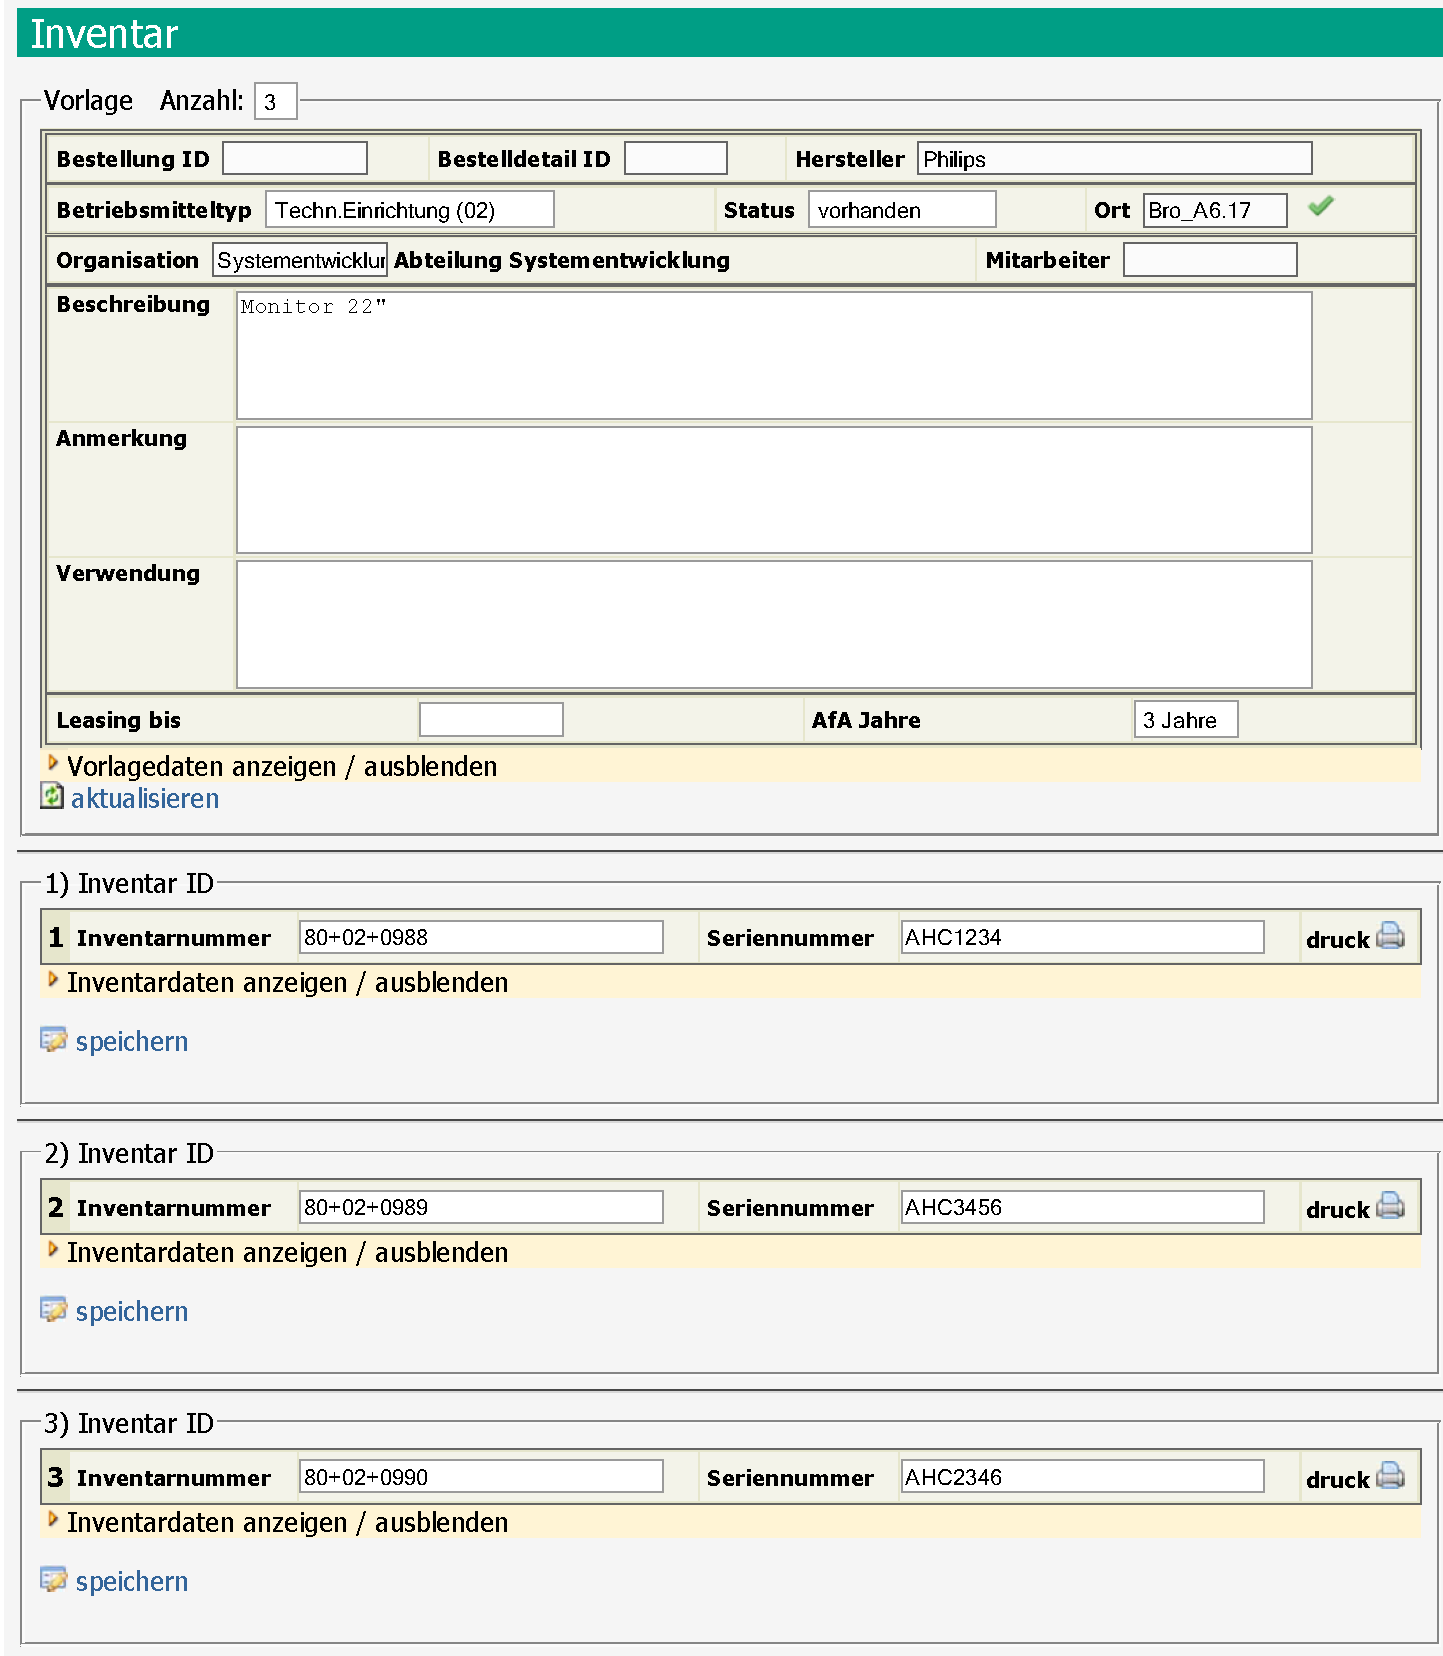
\includegraphics[width=0.80\textwidth]{Inventar_neu.png}
	\caption{Neuanlage}
	\label{Neuanlage}
\end{figure}


\chapter{Suchen und Bearbeiten von Betriebsmitteln}
\label{Suchen und Bearbeiten von Betriebsmitteln}
Um den Inventardatensatz eines Betriebsmittels anzuzeigen, gen�gt es, die Seite Inventar->Suche zu �ffnen, und mithilfe des Barcodescanners den Strichcode einzuscannen. 
Die Betriebsmitteldaten werden automatisch angezeigt.
\begin{figure}
	\centering
	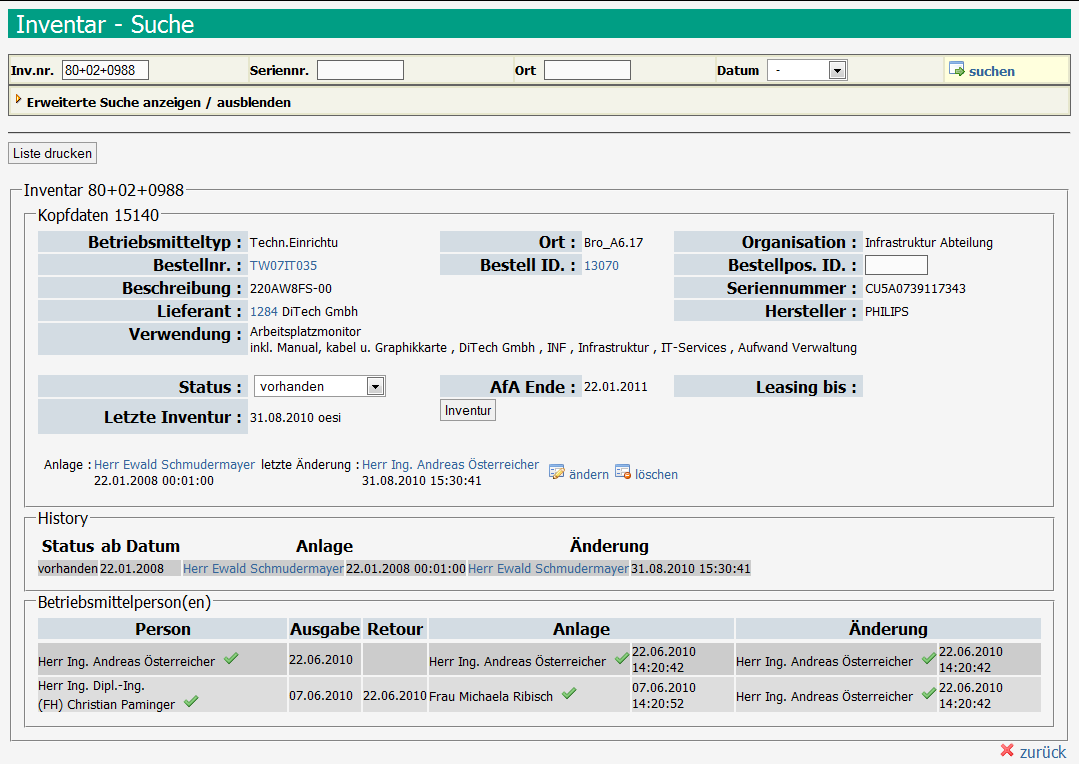
\includegraphics[width=0.80\textwidth]{Inventar_detail.png}
	\caption{Suche nach Betriebsmitteln}
	\label{Suche nach Betriebsmitteln}
\end{figure}

Betriebsmittel k�nnen auch nach Ort, Mitarbeiter, Organisationseinheit, etc gesucht werden.
Klicken Sie auf 'Erweiterte Suche anzeigen' um die Expertensuche einzublenden.

\begin{figure}
	\centering
	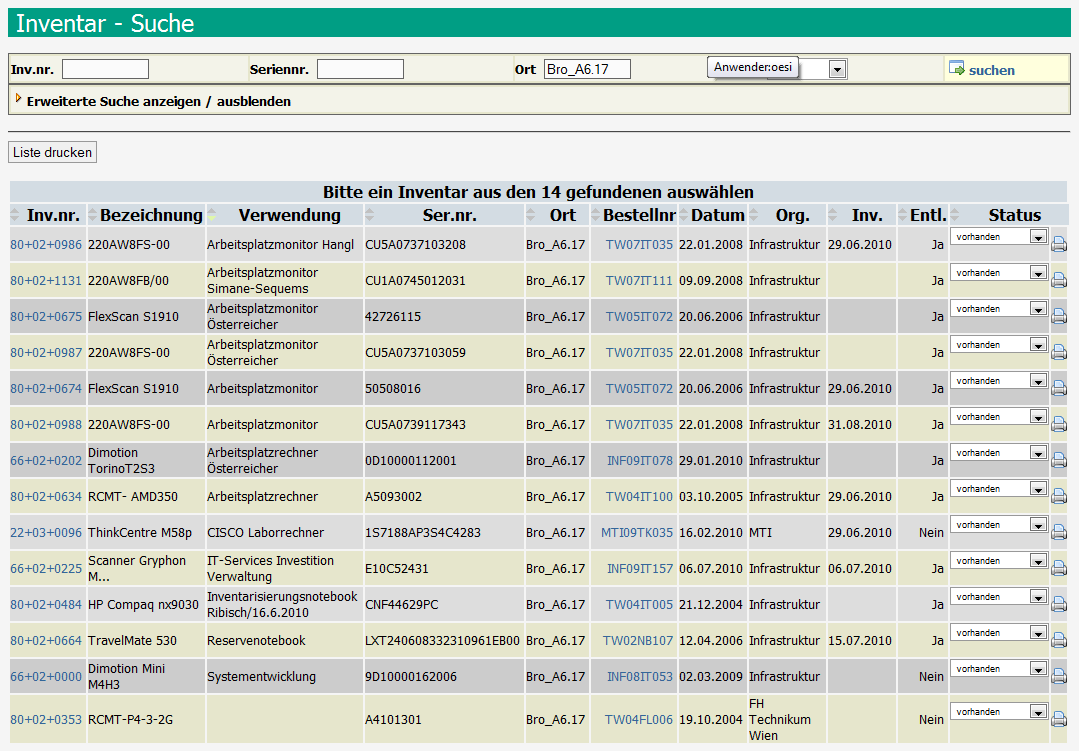
\includegraphics[width=0.80\textwidth]{Inventar_suche.png}
	\caption{Suche nach Betriebsmitteln}
	\label{Suche nach Betriebsmitteln}
\end{figure}

Um die Daten zu bearbeiten klicken Sie auf den Punkt '�ndern'.

\begin{figure}
	\centering
	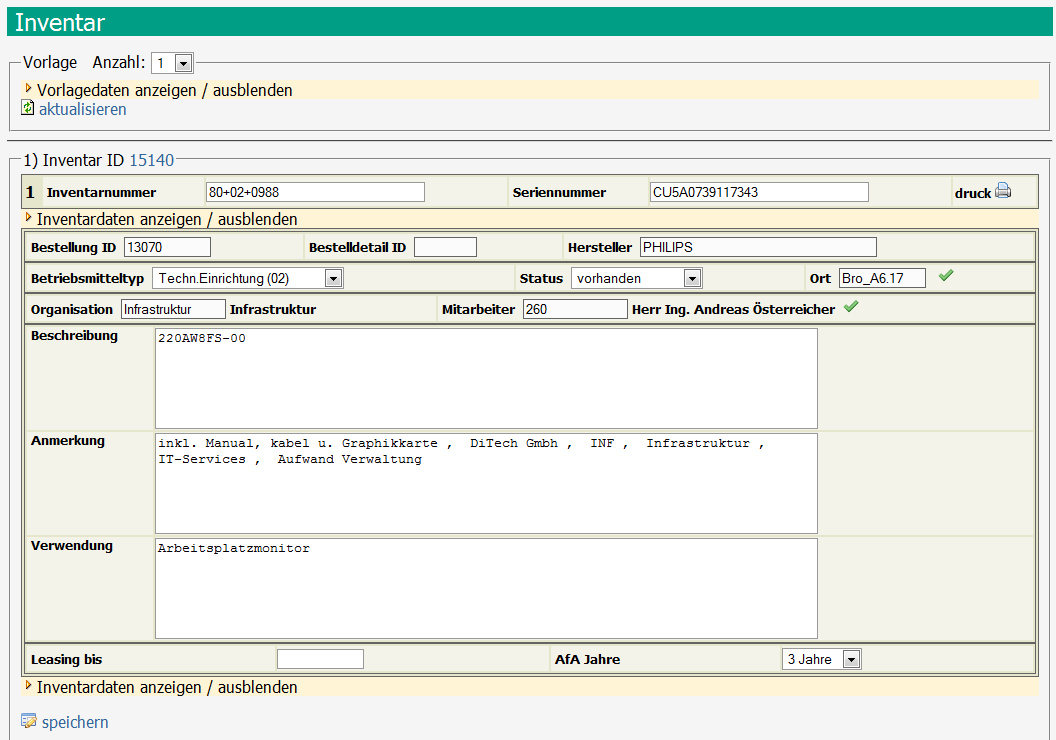
\includegraphics[width=0.80\textwidth]{Inventar_bearbeiten.png}
	\caption{�ndern von Betriebsmitteln}
	\label{�ndern von Betriebsmitteln}
\end{figure}
\chapter{Inventur}
\label{Inventur}
F�r die Inventur der Betriebsmittel steht ein eigenes Tool zur Verf�gung.
Sie finden es unter dem Men�punkt Inventar->Inventur.
Hier k�nnen sie Ausw�hlen f�r welchen Raum und/oder welche Person sie die Inventur durchf�hren.
Klicken Sie auf 'Inventur starten' um zu beginnen.
\begin{figure}
	\centering
	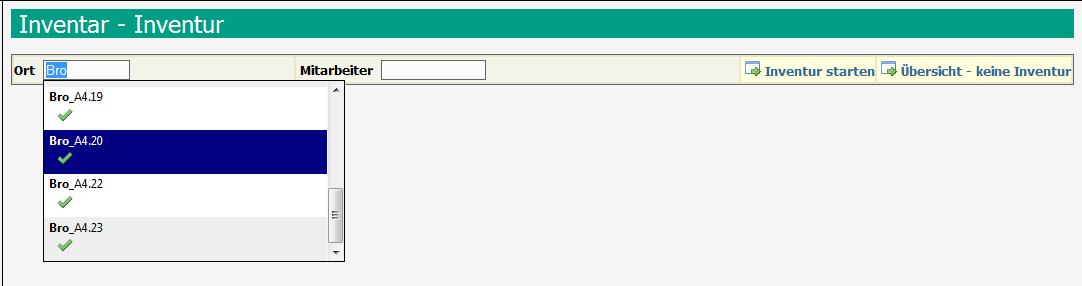
\includegraphics[width=0.80\textwidth]{Inventar_inventur_autocomplete.png}
	\caption{Raumauswahl}
	\label{Raumauswahl}
\end{figure}

Sie k�nnen nun die vorhandenen Betriebsmittel mit dem Barcodescanner nacheinander erfassen.
Bei diesen Betriebsmittel wird nun automatisch das Inventurdatum gesetzt, der Name der Person welche die Inventur durchgef�hrt hat und das Betriebsmittel wird automatisch dem ausgew�hlten Raum und/oder der Person zugeordnet.
\begin{figure}
	\centering
	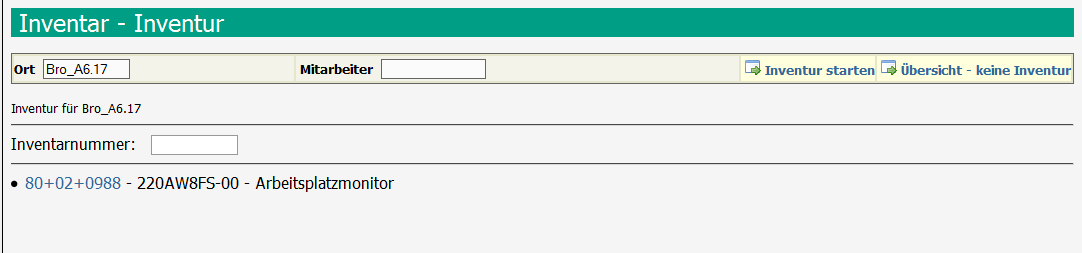
\includegraphics[width=0.80\textwidth]{Inventar_inventur.png}
	\caption{Inventur der Betriebsmittel}
	\label{Inventur der Betriebsmittel}
\end{figure}
\\
Nachdem Sie alle Ger�te in diesem Raum oder von dieser Person erfasst haben, k�nnen Sie sich eine Liste der Ger�te anzeigen lassen, die sich in diesem Raum oder im Besitz der Person befinden sollten, aber in den letzten 20 Wochen nicht erfasst wurden.
Klicken Sie dazu auf den Punkt '�bersicht - keine Inventur'.\\
Sie k�nnen hier die nicht erfassten Ger�te auscheiden oder in einen Dummy-Raum zur weiteren Bearbeitung verschieben.\\
\begin{figure}
	\centering
	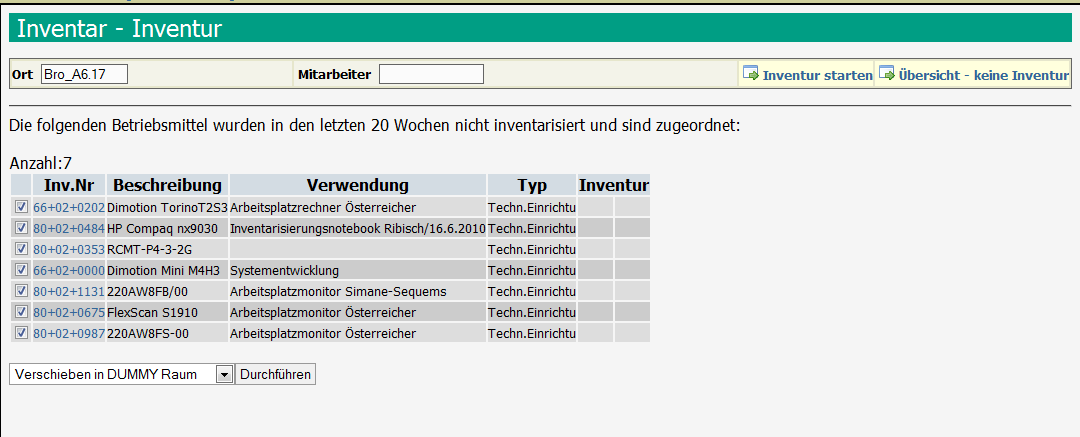
\includegraphics[width=0.80\textwidth]{Inventar_inventur_keine_inventur.png}
	\caption{�bersucht der Betriebsmittel die nicht erfasst wurden}
	\label{�bersicht der Betriebsmittel die nicht erfasst wurden}
\end{figure}

%% Kapitel Ende   %%%%%%%%%%%%%%%%%%%%%%%%%%%%%%%%%%%%%%%%%%%%%%%%%
\appendix							% Beginn des Anhangs
\chapter{Schluss}
\listoftables					% Tabellenverzeichnis
\listoffigures				% Abbildungsverzeichnis
\end{document}
